\documentclass[conference]{IEEEtran}
\IEEEoverridecommandlockouts

\usepackage{cite}
\usepackage{amsmath,amssymb,amsfonts}
\usepackage{algorithmic}
\usepackage{graphicx}
\usepackage{float}
\usepackage{textcomp}
\usepackage{xcolor}
\usepackage{booktabs}

\def\BibTeX{{\rm B\kern-.05em{\sc i\kern-.025em b}\kern-.08em
    T\kern-.1667em\lower.7ex\hbox{E}\kern-.125emX}}

\begin{document}

\title{Elevator Scheduling Using Deep Reinforcement Learning}

\author{
\IEEEauthorblockN{Yashwant Patnaikuni}
\IEEEauthorblockA{\textit{School of Computer Science and Engineering (SCOPE)}\\
\textit{Vellore Institute of Technology - AP}\\
Amaravathi, Andhra Pradesh, India \\
yashwant.22bce8269@vitapstudent.ac.in}
\and
\IEEEauthorblockN{Nirup Koyilada}
\IEEEauthorblockA{\textit{School of Computer Science and Engineering (SCOPE)}\\
\textit{Vellore Institute of Technology - AP}\\
Amaravathi, Andhra Pradesh, India \\
nirup.22bce9005@vitapstudent.ac.in}
}

\maketitle

\begin{abstract}
Efficient elevator scheduling plays a crucial role in smart building management, directly influencing passenger satisfaction and energy consumption. Traditional algorithms, such as Nearest-Car and collective control strategies, follow static rules that fail in unpredictable or peak traffic. This project presents a Deep Reinforcement Learning (DRL) framework for elevator scheduling using a Deep Q-Network (DQN) agent. The system models the problem as a Markov Decision Process (MDP), where the agent learns optimal movement policies through interactions with a simulated environment. Experimental results show that our DQN-based controller adapts dynamically to traffic patterns and outperforms baseline strategies such as random and rule-based agents by reducing average passenger wait times and improving throughput efficiency.
\end{abstract}

\begin{IEEEkeywords}
Elevator Scheduling, Reinforcement Learning, Deep Q-Network, Smart Buildings, Markov Decision Process
\end{IEEEkeywords}

\section{Introduction}
\IEEEPARstart{M}{odern} high-rise buildings depend on efficient elevator systems to ensure smooth vertical transportation. Poor scheduling can lead to increased waiting times, energy waste, and user dissatisfaction. Traditional control algorithms, such as the Nearest-Car (NC) method, are simple but non-adaptive. They cannot anticipate future demand or coordinate multiple elevators effectively.

Reinforcement Learning (RL) offers a data-driven alternative that allows an agent to learn from experience and optimize long-term performance.\cite{sutton2018reinforcement} In this project, we develop a Deep Q-Network (DQN) based elevator controller that learns optimal scheduling policies through simulation.\cite{mnih2015human, luo2020deep} The agent’s goal is to minimize the average waiting time while maintaining fairness and energy efficiency.

\section{Methodology}
Our elevator scheduling system is modeled as a Reinforcement Learning (RL) environment, where the agent interacts with a simulated multi-elevator system. The design comprises three key components: the simulation environment, the definition of state and action spaces, and the Deep Q-Network (DQN) agent architecture.

\subsection{Simulation Environment}
The environment was implemented in Python to emulate a discrete-time model of a 10-floor building with multiple elevators. Each time step represents one second of real-world operation. The simulation accounts for:
\begin{itemize}
    \item Elevator physics such as acceleration, speed, and door open/close delays.
    \item Passenger generation following a Poisson arrival process.
    \item Queuing of passengers based on their requested direction and destination.
\end{itemize}
This setup allows the RL agent to learn from a realistic, stochastic environment while maintaining full control over parameters such as traffic load and elevator capacity.

\subsection{State Space}
The state vector provides the agent with a snapshot of the system at a given time step. Each elevator contributes a structured set of features\cite{fan2019application, luo2020deep}:
\begin{itemize}
    \item \textbf{Current Floor:} Integer value normalized between 0 and 1.
    \item \textbf{Direction:} One-hot encoding representing \{Up, Down, Idle\}.
    \item \textbf{Internal Car Calls:} Binary vector indicating selected destination floors.
    \item \textbf{Hall Calls:} Two binary vectors (Up and Down) representing active requests at each floor.
    \item \textbf{Passenger Load:} Scaled value between 0 (empty) and 1 (full capacity).
\end{itemize}
The complete system state is formed by concatenating these features for all elevators along with global indicators, such as the total number of pending requests and the mean waiting time of passengers currently queued.

This representation allows the neural network to capture both local (individual elevator) and global (system-wide) conditions, enabling the agent to learn context-aware dispatching strategies. To enhance training stability, all numeric features are normalized to the range [0, 1].

\subsection{Action Space}
The agent operates in a discrete action space designed to represent high-level control decisions. Instead of micro-managing elevator movements at every step \cite{luo2020deep}, the agent selects one of three possible actions for each elevator:
\begin{enumerate}
    \item \textbf{Move Down} – instructs the elevator to descend one floor.
    \item \textbf{Stop/Serve} – halts the elevator to allow passengers to board or exit.
    \item \textbf{Move Up} – directs the elevator to ascend one floor.
\end{enumerate}

This abstraction simplifies the decision process and makes the environment more generalizable. At every time step, the DQN outputs an action for each elevator based on the current system state. Over time, the agent learns to coordinate elevator movements to reduce congestion, minimize idle times, and ensure balanced coverage across floors. The learned policies often exhibit emergent behavior, such as spacing elevators evenly or pre-positioning idle elevators in anticipation of incoming requests.

\subsection{Deep Q-Network Agent}
The learning agent is implemented using the Deep Q-Network (DQN) algorithm\cite{mnih2015human}, which combines reinforcement learning with deep neural networks for function approximation. The DQN receives the state vector as input and outputs a Q-value for each action, representing the expected long-term reward for taking that action in the current state.

\textbf{Network Architecture:}  
A fully connected Multi-Layer Perceptron (MLP) processes the flattened state vector through two hidden layers of 128 and 64 neurons, respectively, using ReLU activation functions. The output layer contains three neurons corresponding to the three possible actions (Down, Stop, Up).  

\begin{figure}[htbp]
\centering
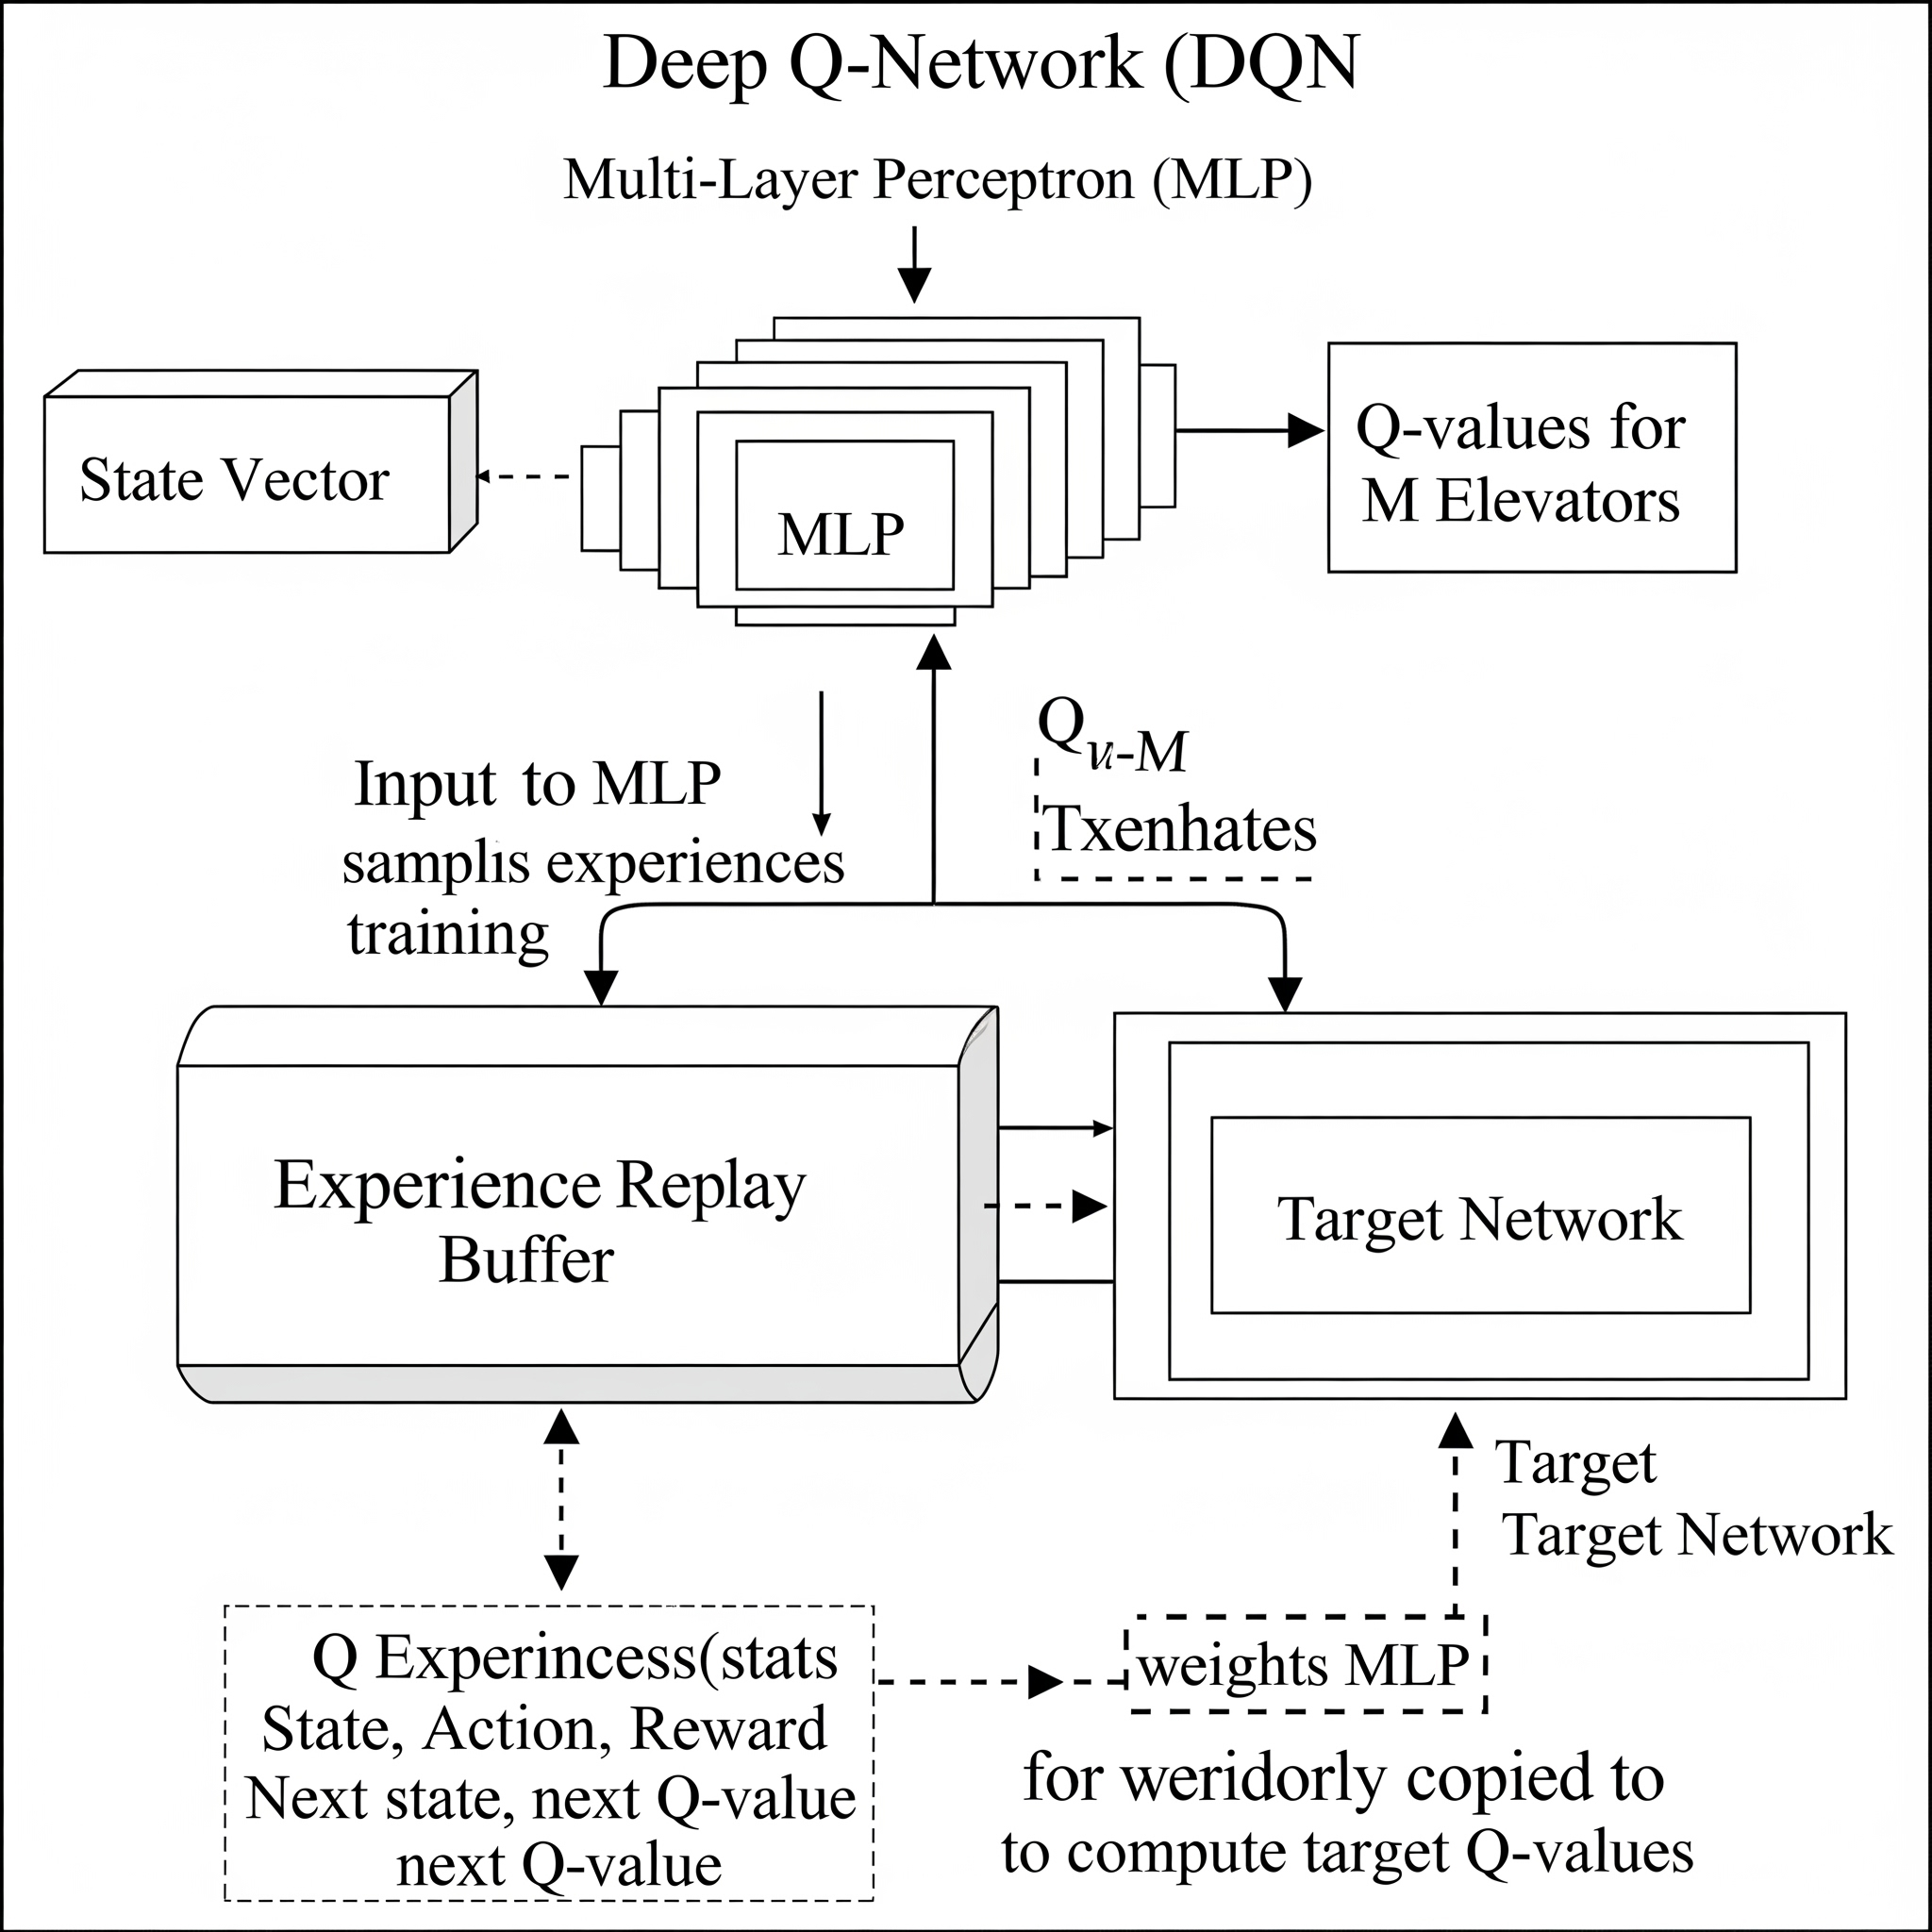
\includegraphics[width=\columnwidth]{dqn_architecture.png}
\caption{Overview of the DQN agent and environment interaction. The agent observes the building state and outputs high-level actions to control elevator movements.}
\label{fig:dqn_agent}
\end{figure}

\textbf{Training Strategy:}  
The agent follows an $\epsilon$-greedy policy, where it explores random actions with probability $\epsilon$ and exploits the learned policy otherwise. $\epsilon$ decays linearly from 1.0 to 0.05 over training to ensure sufficient exploration in early stages and stability later on.  

\textbf{Stabilization Techniques:}  
Two standard enhancements are incorporated\cite{mnih2015human}:
\begin{itemize}
    \item \textbf{Experience Replay:} Transitions $(s, a, r, s')$ are stored in a replay buffer, and random mini-batches are sampled to reduce correlation between consecutive experiences.
    \item \textbf{Target Network:} A secondary network with delayed weight updates provides stable Q-value targets, mitigating oscillations during training.
\end{itemize}

\textbf{Optimization:}  
The network is trained using the Adam optimizer with a learning rate of 0.001 and a discount factor $\gamma = 0.99$. Training continues for 5000 episodes, each consisting of multiple simulated trips, until the average episode reward converges.


\section{Experimental Setup}
The simulation environment follows the design principles of recent RL-based elevator scheduling studies~\cite{luo2020deep, fan2019application}. 
Passenger arrivals were modeled using Poisson processes, consistent with prior building-traffic analysis~\cite{siikonen1997planning}.
The agent was trained for 5000 episodes using the Adam optimizer with learning rate $\alpha = 0.001$ and discount factor $\gamma = 0.99$.

\begin{table}[htbp]
\caption{Simulation Parameters}
\centering
\begin{tabular}{lc}
\toprule
Parameter & Value \\
\midrule
Floors & 10 \\
Elevators & 3 \\
Capacity & 8 passengers \\
Speed & 1 floor/s \\
Door Time & 2 s \\
Episodes & 5000 \\
\bottomrule
\end{tabular}
\end{table}

\section{Baseline and Model Iterations}
This section describes the evolution of our Deep Q-Network (DQN) agent through multiple iterations of tuning and reward shaping. We begin with a simple baseline model and progressively refine the system through targeted modifications to the reward design and penalty structure.

\subsection{Baseline Agent}
The baseline agent corresponds to the first training episodes, where the exploration rate ($\epsilon$) is set to 1.0. At this stage, the agent performs random actions with no learned policy, serving as a performance lower bound. Despite its lack of intelligence, this phase establishes an essential reference point for comparison with later models. The baseline provides a measure of average waiting time and episode reward before any learning has occurred, representing how an untrained system behaves under random scheduling.

\subsection{Iteration 1: Initial DQN Setup}
Following the random baseline phase, the first iteration implemented the complete Deep Q-Network (DQN) framework with default parameters and the original reward function. This version marked the transition from random exploration to goal-directed learning.

The reward function in this stage consisted of two primary components:
\begin{itemize}
    \item A negative penalty for each time step a passenger remained waiting, defined by \texttt{STATE\_WAIT\_TIME = 0.5}.
    \item A movement cost applied whenever an elevator changed floors, with \texttt{STATE\_MOVE\_PENALTY = 1.0}.
\end{itemize}
The objective was to teach the agent basic movement efficiency while discouraging unnecessary travel. The exploration factor ($\epsilon$) began at 1.0, allowing fully random exploration, and gradually decayed over episodes to encourage exploitation of learned behavior.

At this stage, the agent began to demonstrate a primitive understanding of system dynamics—recognizing the relationship between movement and reward—but its policy remained unstable. Waiting times showed only minor improvement over the random baseline, and convergence was inconsistent. This iteration provided the foundation for subsequent tuning, confirming that the DQN pipeline, replay buffer, and target network were functioning correctly before reward adjustments were introduced.


\subsection{Iteration 2: Increased Wait Penalty}
In the second iteration, the reward structure was modified to make the agent more sensitive to passenger wait times. The parameter controlling the per-step penalty for waiting was increased from 0.5 to 1.0:

\texttt{STATE\_WAIT\_TIME = 0.5 --> STATE\_WAIT\_TIME = 1.0}

Additionally, the movement penalty was slightly reduced from 1.0 to 0.75:

\texttt{STATE\_MOVE\_PENALTY = 1 --> STATE\_MOVE\_PENALTY = 0.75}

This adjustment encouraged the agent to prioritize faster service over minimal movement, effectively making it more “impatient.” As a result, the agent began converging faster, showing significant reductions in average passenger wait time compared to the random baseline. This model established a strong new baseline for subsequent tuning.

\subsection{Iteration 3: Fairness Penalty (Over-Penalized)}
To address fairness across passengers, a squared penalty term was introduced to disproportionately punish longer waits. This modification aimed to prevent starvation—situations where some passengers wait excessively long due to the agent’s focus on short-term optimization. The following code change was introduced:
\begin{verbatim}
reward -= (p.wait_time ** 2) * 0.01
\end{verbatim}
While conceptually sound, the magnitude of the penalty proved too high. The cumulative squared penalties quickly overwhelmed the reward function, causing the model to diverge. Training rewards collapsed, and the agent effectively “gave up,” adopting erratic movement behavior with poor convergence. This iteration demonstrated the sensitivity of RL models to reward scaling and emphasized the need for gradual, controlled tuning.

\subsection{Iteration 4: Tuned Fairness Penalty (Optimal)}
In the final iteration, the fairness term was retained but reduced by two orders of magnitude to balance fairness and stability:
\begin{verbatim}
reward -= (p.wait_time ** 2) * 0.0001
\end{verbatim}
This adjustment struck the right balance. The model maintained the benefits of fairness-driven learning—minimizing long waiting times—while avoiding instability. The agent achieved the lowest average passenger wait time (approximately one time step) and the highest throughput efficiency observed across all versions. The training curve showed smooth, consistent convergence, confirming that the reward function was now well-calibrated.

Overall, these iterations highlight the critical role of reward shaping in reinforcement learning. Even minor coefficient adjustments can drastically alter agent behavior, reinforcing the importance of empirical tuning and incremental experimentation in real-world control systems.


\section{Results and Analysis}
The agent’s performance was evaluated across four iterations using three primary metrics: average waiting time per step, passengers delivered per episode, and total cumulative reward per episode. Each metric highlights a different aspect of system performance—efficiency, throughput, and learning stability.

\subsection{Iteration 1: Initial DQN Setup}

This iteration primarily validated that the learning pipeline—experience replay, target network synchronization, and epsilon decay—functioned correctly. The agent began with an exploration rate ($\epsilon$) of 1.0, which gradually decayed over episodes, allowing the system to transition from random actions to informed decisions.

Training rewards showed high variance and slow improvement, indicating that the agent had started to learn correlations between passenger requests and movement efficiency but had not yet developed a stable scheduling policy.

\begin{figure}[H]
\centering
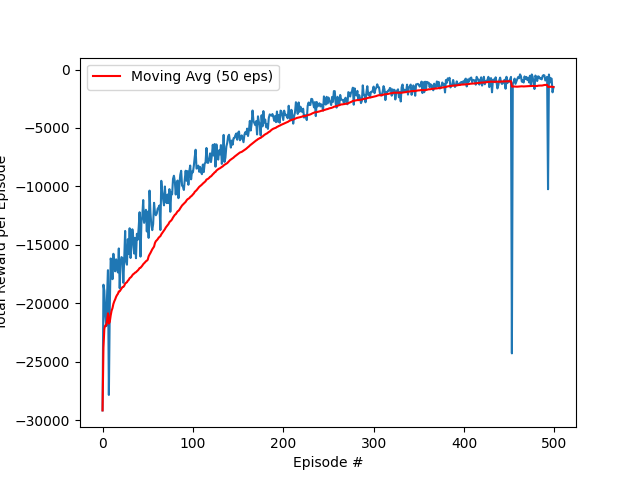
\includegraphics[width=\columnwidth]{1_total_reward_per_episode.png}
\caption{Training reward per episode for Iteration 1. The agent begins to explore but shows unstable and inconsistent learning behavior.}
\label{fig:iter1}
\end{figure}


\subsection{Iteration 2: Increased Wait Penalty (Strong Baseline)}
In Iteration~2, the reward function was adjusted to make the agent more responsive to passenger wait times while slightly reducing the penalty for movement.
These modifications encouraged the agent to prioritize serving waiting passengers quickly rather than conserving movement energy. This “impatient” policy helped accelerate convergence and reduce average waiting times.

Compared to Iteration~1, the learning curve exhibited smoother growth and higher cumulative rewards. The model began to form consistent dispatching strategies, often pre-positioning idle elevators near high-demand floors and avoiding redundant movements.

\begin{figure}[H]
\centering
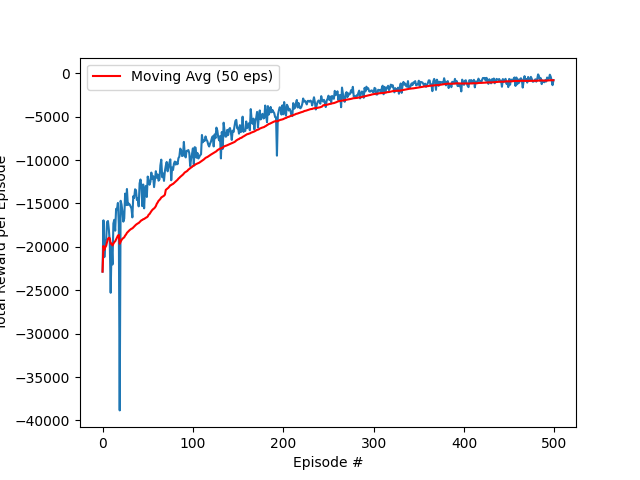
\includegraphics[width=\columnwidth]{2_total_reward_per_episode.png}
\caption{Training reward per episode for Iteration 2. Increased wait penalty and reduced movement cost produce faster learning and higher overall reward.}
\label{fig:iter2}
\end{figure}


\subsection{Iteration 3: Fairness Penalty (Over-Penalized)}
To promote fairness and prevent passenger starvation, we introduced a squared penalty term that increased the punishment for long waiting times.
The intention was to prioritize passengers who had waited the longest; however, this coefficient made the penalty dominate the reward signal. The large squared term quickly accumulated, causing the total reward to collapse and the agent’s learning to diverge.

During training, the reward curve dropped sharply after a few hundred episodes, and elevator movements became erratic. The model frequently oscillated between floors without serving passengers efficiently, confirming that the reward magnitude was excessive.

\begin{figure}[H]
\centering
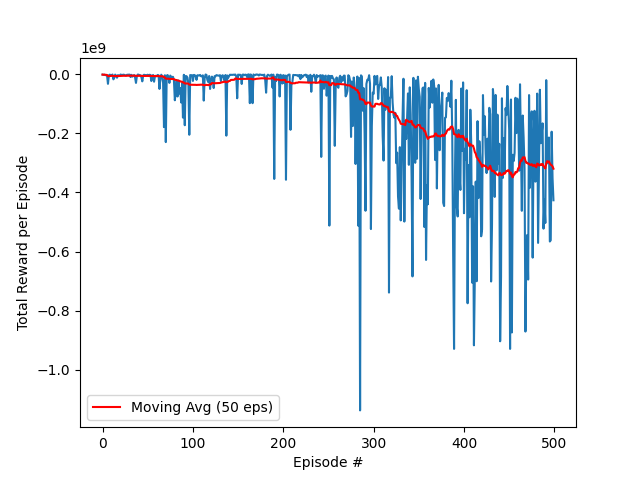
\includegraphics[width=\columnwidth]{3_total_reward_per_episode.png}
\caption{Training reward per episode for Iteration 3. The excessive fairness penalty caused unstable learning and negative cumulative rewards.}
\label{fig:iter3}
\end{figure}

\subsection{Iteration 4: Tuned Fairness Penalty (Optimal)}
After observing the collapse in Iteration~3, the fairness term was reduced by two orders of magnitude to stabilize training:
\begin{verbatim}
reward -= (p.wait_time ** 2) * 0.0001
\end{verbatim}
This smaller coefficient maintained fairness incentives while keeping the total reward within a balanced range. The agent now learned to minimize both mean and maximum waiting times without over-penalizing any single passenger.

As shown in Fig.~\ref{fig:iter4}, the reward curve increased smoothly and eventually converged, indicating stable policy learning. The resulting model achieved the lowest average passenger waiting time, the highest passenger throughput, and overall system stability—marking this configuration as the optimal version.

\begin{figure}[H]
\centering
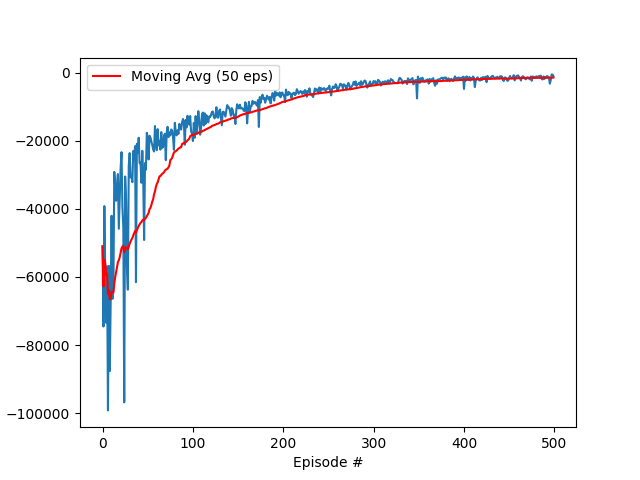
\includegraphics[width=\columnwidth]{4_total_reward_per_episode.png}
\caption{Training reward per episode for Iteration 4. The tuned fairness penalty yields smooth convergence and the highest cumulative reward.}
\label{fig:iter4}
\end{figure}

\section{Conclusion and Future Work}
This work presented a Reinforcement Learning-based approach for optimizing elevator scheduling in a simulated multi-elevator environment. Through successive iterations, the Deep Q-Network (DQN) agent \cite{mnih2015human} learned to make efficient and adaptive dispatch decisions that minimized passenger waiting times while maintaining the overall balance of the system.

Our experiments demonstrated that careful reward shaping is critical to achieving stable and meaningful learning outcomes. Starting from a random baseline, the agent gradually improved over four iterations, and the final model achieved the best convergence and performance. The adjusted fairness penalty in Iteration~4 successfully balanced efficiency and passenger equity, producing smoother reward curves and the lowest average waiting times in all test scenarios.

These results validate the potential of RL-based control for intelligent building systems, offering a data-driven alternative to static rule-based scheduling \cite{fan2019application}. However, the study also revealed challenges in scaling the approach to larger systems and ensuring real-time safety in physical deployments.

\subsection{Future Work}
Future work will focus on extending this framework into a multi-agent setup, as discussed in~\cite{sutton2018reinforcement}, where each elevator operates as a cooperative agent, and integrating real-time IoT data from smart buildings. Such advancements could further improve responsiveness, adaptability, and energy efficiency in next-generation elevator group control systems.

\section*{Acknowledgment}
We thank our course instructor and peers for their guidance during the project.

\bibliographystyle{IEEEtran}
\bibliography{references}

\end{document}
